\documentclass[a4]{article}
\pagestyle{myheadings}

%%%%%%%%%%%%%%%%%%%
% Packages/Macros %
%%%%%%%%%%%%%%%%%%%
\usepackage{mathrsfs}


\usepackage{fancyhdr}
\pagestyle{fancy}
\lhead{}
\chead{}
\rhead{}
\lfoot{}
\cfoot{} 
\rfoot{\normalsize\thepage}
\renewcommand{\headrulewidth}{0pt}
\renewcommand{\footrulewidth}{0pt}
\newcommand{\RomanNumeralCaps}[1]
{\MakeUppercase{\romannumeral #1}}

\usepackage{amssymb,latexsym}  % Standard packages
\usepackage[utf8]{inputenc}
\usepackage[russian]{babel}
\usepackage{MnSymbol}
\usepackage{amsmath,amsthm}
\usepackage{indentfirst}
\usepackage{graphicx}%,vmargin}
\usepackage{graphicx}
\graphicspath{{pictures/}} 
\usepackage{verbatim}
\usepackage{color}









\DeclareGraphicsExtensions{.pdf,.png,.jpg}% -- настройка картинок

\usepackage{epigraph} %%% to make inspirational quotes.
\usepackage[all]{xy} %for XyPic'a
\usepackage{color} 
\usepackage{amscd} %для коммутативных диграмм


\newtheorem{Lemma}{Лемма}[section]
\newtheorem{Proposition}{Предложение}[section]
\newtheorem{Theorem}{Теорема}[section]
\newtheorem{Corollary}{Следствие}[section]
\newtheorem{Remark}{Замечание}[section]
\newtheorem{Definition}{Определение}[section]
\newtheorem{Designations}{Обозначение}[section]




%%%%%%%%%%%%%%%%%%%%%%%% 
%Сношение с оглавлением% 
%%%%%%%%%%%%%%%%%%%%%%%% 
\usepackage{tocloft} 
\renewcommand{\cftdotsep}{2} %частота точек
\renewcommand\cftsecleader{\cftdotfill{\cftdotsep}}
\renewcommand{\cfttoctitlefont}{\hspace{0.38\textwidth} \LARGE\bfseries} 
\renewcommand{\cftsecaftersnum}{.}
\renewcommand{\cftsubsecaftersnum}{.}
\renewcommand{\cftbeforetoctitleskip}{-1em} 
\renewcommand{\cftaftertoctitle}{\mbox{}\hfill \\ \mbox{}\hfill{\footnotesize Стр.}\vspace{-0.5em}} 
\renewcommand{\cftsubsecfont}{\hspace{1pt}} 
\renewcommand{\cftparskip}{3mm} %определяет величину отступа в оглавлении
\setcounter{tocdepth}{5} 




\addtolength{\textwidth}{0.7in}
\textheight=630pt
\addtolength{\evensidemargin}{-0.4in}
\addtolength{\oddsidemargin}{-0.4in}
\addtolength{\topmargin}{-0.4in}

\newcommand{\empline}{\mbox{}\newline} 
\newcommand{\likechapterheading}[1]{ 
	\begin{center} 
		\textbf{\MakeUppercase{#1}} 
	\end{center} 
	\empline} 

\makeatletter 
\renewcommand{\@dotsep}{2} 
\newcommand{\l@likechapter}[2]{{\bfseries\@dottedtocline{0}{0pt}{0pt}{#1}{#2}}} 
\makeatother 
\newcommand{\likechapter}[1]{ 
	\likechapterheading{#1} 
	\addcontentsline{toc}{likechapter}{\MakeUppercase{#1}}} 





\usepackage{xcolor}
\usepackage{hyperref}
\definecolor{linkcolor}{HTML}{000000} % цвет ссылок
\definecolor{urlcolor}{HTML}{AA1622} % цвет гиперссылок

\hypersetup{pdfstartview=FitH,  linkcolor=linkcolor,urlcolor=urlcolor, colorlinks=true}



\def \newstr {\medskip \par \noindent} 



\begin{document}
	\def\contentsname{\LARGE{Содержание}}
	\thispagestyle{empty}
	\begin{center} 
		\vspace{2cm} 
		{\Large \sc Санкт-Петербургский Политехнический Университет}\\
		\vspace{2mm}
		{\Large\sc Петра Великого}\\
		\vspace{1cm}
		{\large \sc Институт прикладной математики и механики\\ 
			\vspace{0.5mm}
			\textsc{}}\\ 
		\vspace{0.5mm}
		{\large\sc Кафедра $"$Прикладная математика$"$}\\
		\vspace{15mm}
		
		
		{\sc \textbf{Отчёт\\
			Лабораторная работа №$6$\\
			по дисциплине\\
			"Математическая статистика"}
			\vspace{6mm}
			
		}
		\vspace*{2mm}
		
		
		\begin{flushleft}
			\vspace{4cm}
			\sc Выполнил студент:\\
			\sc Салихов С.Р.\\
			\sc группа: 3630102/70401\\
			\vspace{1cm}
			\sc Проверил:\\
			\sc к.ф-м.н., доцент\\
			\sc Баженов Александр Николавич
			\vspace{20mm}
		\end{flushleft}
	\end{center} 
	\begin{center}
		\vfill {\large\textsc{Санкт-Петербург}}\\ 
		2020 г.
	\end{center}
	
	\newpage
	\pagestyle{plain}
	
	%\begin{center}
	%\begin{abstract} 
	
	%\end{abstract}
	
	%\end{center}
	
	\newpage
	\tableofcontents{}
	\newpage
	\listoffigures
	\newpage
	
	
	\section{Постановка задачи}
		Найти оценки коэффициентов линейной регрессии $y_i = a + bx_i + e_i$, используя 20 точек на отрезке $[-1.8; 2]$ с равномерным шагом равным 0.2. Ошибку $e_i$ считать нормально распределённой с параметрами (0, 1). В качестве эталонной зависимости взять $y_i = 2 + 2x_i + e_i$. При построении оценок коэффициентов использовать два критерия: критерий наименьших квадратов и критерий наименьших модулей. Проделать то же самое для выборки, у которой в значения $y_1$ и $y_20$ вносятся возмущения 10 и -10.
	\section{Теория}
		\subsection{Простая линейная регрессия}
		\subsubsection{Модель простой линейной регрессии}
			Регрессионную модель описания данных называют простой линейной регрессией, если
			$$y_i = \beta_0 + \beta_1x_i + \epsilon_i$$ , i = 1, ... , n, где $x_1$, ... , $x_n$ — заданные числа (значения фактора); $y_1$, ... ,$y_n$  — наблюдаемые значения отклика; $\epsilon_1$, ... , $\epsilon_n$ — независимые, нормально распределённые N(0, $\delta$) с нулевым математическим ожиданием и одинаковой (неизвестной) дисперсией случайные величины (ненаблюдаемые); $\beta_0, \beta_1$ — неизвестные параметры, подлежащие оцениванию.\\
			В модели отклик y зависит зависит от одного фактора x, и весь разброс экспериментальных точек объясняется только погрешностями наблюдений (результатов измерений) отклика y. Погрешности результатов измерений x в этой модели полагают существенно меньшими погрешностей результатов измерений y, так что ими можно пренебречь.

		\subsection{Метод наименьших квадратов}
			При оценивании параметров регрессионной модели используют различные методы. Один из наиболее распрстранённых подходов заключается в следующем: вводится мера (критерий) рассогласования отклика и регрессионной функции, и оценки параметров регрессии определяются так, чтобы сделать это рассогласование наименьшим. Достаточно простые расчётные формулы для оценок получают при выборе критерия в виде суммы квадратов отклонений значений отклика от значений регрессионной функции (сумма квадратов остатков):
			$$Q(\beta_0, \beta_1) = \sum_{i = 1}^{n} \epsilon^2_i = \sum_{i = 1}^{n} (y_i - \beta_0 - \beta_1 x_i)^2 -> min_{\beta_0, \beta_1} .$$
			Задача минимизации квадратичного критерия (10) носит название задачи метода наименьших квадратов (МНК), а оценки $\hat{\beta_0}$, $\hat{\beta_1}$ параметров $\beta_0$, $\beta_1$, реализующие минимум критерия, называют МНК-оценками.
		\subsubsection{Расчётные формулы для МНК-оценок}
			МНК-оценки параметров $\hat{\beta_0}$ и $\hat{\beta_1}$ находятся из условия обращения функции Q($\beta_0$, $\beta_1$) в минимум.\\	
			Для нахождения МНК-оценок $\hat{\beta_0}$ и $\hat{\beta_1}$ выпишем необходимые условия экстремума:

			
			\begin{equation*} 
			\begin{cases}
			\frac{\partial Q}{\partial \beta_0} = -2 \sum_{i = 1}^{n} (y_i - \beta_0 - \beta_1 x_i) = 0\\
			\frac{\partial Q}{\partial \beta_1} = -2 \sum_{i = 1}^{n} (y_i - \beta_0 - \beta_1 x_i)x_i = 0
			\end{cases}
			\end{equation*}
			
			Далее для упрощения записи сумм будем опускать индекс суммирования. Из системы получим
			
			\begin{equation*} 
			\begin{cases}
			n\hat{\beta_0} + \hat{\beta_1} \sum x_i = \sum y_i\\
			\hat{\beta_0}\sum x_i + \hat{\beta_1} \sum x^2_i = \sum x_i y_i
			\end{cases}
			\end{equation*}
			
			$$\overline{x} = \frac{1}{n} \ sum x_i, \overline{y} = \frac{1}{n} \ sum y_i, \overline{x^2} = \frac{1}{n} \ sum x^2_i, \overline{xy} = \frac{1}{n} \ sum x_iy_i$$
			Тогда:
			\begin{equation*} 
			\begin{cases}
			\hat{\beta_0} + \hat{\beta_1}\overline{x} = \overline{y}\\
			\hat{\beta_0}\overline{x} + \hat{\beta_1} \overline{x^2} = \overline{xy}
			\end{cases}
			\end{equation*}
			
			откуда МНК-оценку $\hat{\beta_1}$ наклона прямой регрессии находим по формуле
			Крамера
			$$\hat{\beta_1} = \frac{\overline{xy} - \overline{x} * \overline{y}}{\overline{x^2} - {\overline{x}}^2}$$
			а МНК-оценку $\hat{\beta_0}$ определяем непосредственно из первого уравнения системы:
			$$\hat{\beta_0} = \overline{y} - \overline{x}\hat{\beta_1}$$
			
			\subsection{Метод наименьших модулей}
			Критерий наименьших модулей – заключается в минимизации следующей функции \cite{6_4}:
			\begin{equation}
			M(a,b) = \sum\limits_{i=1}^n\vert y_i-ax_i-b\vert\to\min\hfill
			\end{equation}			
			
	\section{Реализация}
	Для генерации выборки был использован $Python\;3.7$ и модуль numpy. Для отрисовки графиков использовался модуль matplotlib. scipy.stats для обработки функций распределений.
	\newpage
	\section{Результаты}
		\begin{figure}[h!]
			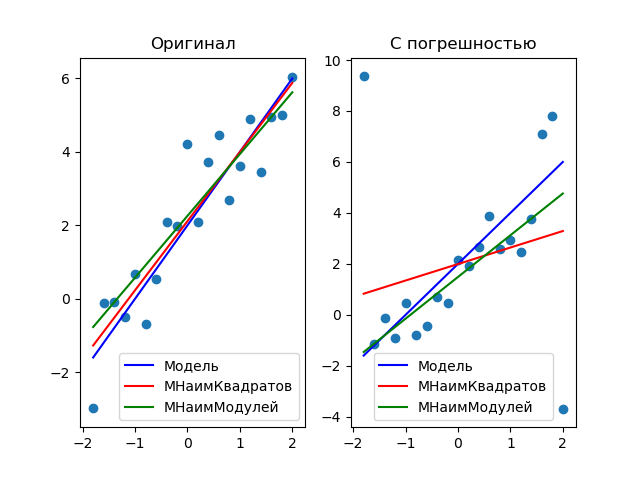
\includegraphics[width=\textwidth]{Graph.png} 
			\caption[Графики линейной регрессии при выборке с возмущением и без]{Графики линейной регрессии при выборке с возмущением и без}
		\end{figure}
		
		\subsection{Выборка без возмущений}
			Критерий наименьших квадратов:\\
			$$\hat{a} \approx 1.93,\hat{b} \approx 2.19$$\\
			
			Критерий наименьших модулей:\\
			$$\hat{a} \approx 2.24 ,\hat{b} \approx 1.77$$
		\subsection{Выборка с возмущниями}
			Критерий наименьших квадратов:\\
			$$\hat{a} \approx 0.48,\hat{b} \approx 1.76$$\\
			
			Критерий наименьших модулей:\\
			$$\hat{a} \approx 1.85 ,\hat{b} \approx 1.39$$
		
	\section{Обсуждение}
		1)МНК оценивает коэффициенты линейной регрессии точнее, на выборке без возмущений.\\
		Для доказательства этого введём метрику суммы квадратов разностей значений по оси y между МНК и модели и МНМ и модели. $\rho_1$ = $\sum (y_{MNK} - y_{etl})^2$ , $\rho_2$ = $\sum (y_{MNM} - y_{etl})^2$ и увидим, что $\rho_1$ всегда меньше $\rho_2$.\\ 
		\begin{center}
			Пример: \\
			$y_{etl}$ = [-1.60, -1.20, -0.80, -0.40,  0.00,   0.40,  0.80, 1.20,  1.60,  2.00,   2.40,  2.80,  3.20,  3.60, 4.00,  4.40,  4.80,  5.20,  5.60,  6.0 ]\\
			$y_{MNK} \approx $ [-1.27, -0.89, -0.52,  -0.14,  0.23,  0.61, 0.98,  1.36,  1.74,  2.11,  2.491,  2.86, 3.24,  3.62  3.99   4.37,  4.75, 5.12, 5.50  5.85]\\
			$y_{MNM} \approx$ [-0.77, -0.43, -0.09,  0.23,  0.57,  0.911,  1.24,  1.58,  1.92,  2.25,  2.59,  2.93,  3.26,  3.60,  3.94,  4.27,  4.61,  4.95,  5.28,  5.62]\\
			
			МНК : $\hat{a}$ = 1.88, $\hat{b}$ = 2.11\\
			МНМ : $\hat{a}$ = 2.26, $\hat{b}$ = 1.68\\
			
			$\rho_1$ = 16.59\\
			$\rho_2$ = 17.96\\
			
			Таким образом, $\rho_1$ < $\rho_2$.
		\end{center}
		
		2)На выборке с возмущениями эффективнее использовать МНМ. Таким образом, метод наименьших модулей устойчив к редким выбросам, в свою очередь МНМ обладает большей сложностью вычислений, чем МНК(т.к. ,в коде, МНК - оценки вычисляются из расчётных формул, а МНМ - оценки вычисляются, через решение задачи минимизации).
		
	\section{Литература}
	
	\href{https://physics.susu.ru/vorontsov/language/numpy.html}{Модуль numpy}\\
	
	\href{https://matplotlib.org/}{Модуль matplotlib}\\
	
	\href{https://www.scipy.org/}{Модуль scipy}\\
	
	\href{https://ru.wikipedia.org/wiki/%D0%9C%D0%B5%D1%82%D0%BE%D0%B4_%D0%BD%D0%B0%D0%B8%D0%BC%D0%B5%D0%BD%D1%8C%D1%88%D0%B8%D1%85_%D0%BC%D0%BE%D0%B4%D1%83%D0%BB%D0%B5%D0%B9}{Метод наименьших модулей}\\
	
	\href{https://ru.wikipedia.org/wiki/%D0%9C%D0%B5%D1%82%D0%BE%D0%B4_%D0%BD%D0%B0%D0%B8%D0%BC%D0%B5%D0%BD%D1%8C%D1%88%D0%B8%D1%85_%D0%BA%D0%B2%D0%B0%D0%B4%D1%80%D0%B0%D1%82%D0%BE%D0%B2}{Метод наименьших квадратов}\\
	
	\section{Приложения}
	
	\href{https://github.com/LuciusGen/Matstat/blob/master/Lab6/Lab6.py}{Код лаборатрной}
	
	\href{https://github.com/LuciusGen/Matstat/blob/master/Lab6/lab6.tex}{Код отчёта}
	
\end{document}